\chapter{Здоровье}

\section{Средиземноморская диета}
\textit{Источник: \url{https://oberig.ua/ru/news/statti/seredzemnomorska-dijeta-185}}

\textbf{Что она предполагает и почему полезна?} Средиземноморская диета – это план правильного питания, который содержит много фруктов и овощей, цельнозерновых продуктов, рыбы и оливкового масла. Средиземноморская диета снижает риск сердечно-сосудистых заболеваний, некоторых видов рака, сахарного диабета, болезни Альцгеймера и Паркинсона. Также она помогает сбросить лишний вес.

Включает ли средиземноморская диета пиццу с колбасками и большие порции спагетти? К сожалению, нет! Первым популяризатором средиземноморской диеты был американский ученый Ансель Кис. В середине ХХ столетия он обнаружил, что жители Крита и юга Италии имели хорошее состояние сердечно-сосудистой системы в отличие от населения США.

Они питались свежими продуктами преимущественно растительного происхождения и занимались физическим трудом. Говоря о средиземноморской диете, надо понимать, что это традиционная диета средиземноморских стран, а не ее современный «ресторанный» вариант.

Четкого перечня продуктов, которые включает средиземноморская диета, не существует. Это ориентировочный план здорового питания, который можно корректировать согласно своим возможностям и предпочтениям. Кухни средиземноморских стран очень разнообразны, но все они разделяют общие принципы:

\begin{enumerate}
    \item Преимущественно растительная пища (фрукты и овощи; паста, каши и хлеб из цельного зерна; бобовые и орехи);
    \item Замена сливочного масла на оливковое масло;
    \item Использование трав и специй вместо соли для улучшения вкуса пищи;
    \item Снижение употребления красного мяса до 1-2 раз в месяц;
    \item Рыба и птица – 2 раза в неделю;
    \item Умеренное употребление вина;
    \item Достаточная физическая активность.
\end{enumerate}

Средиземноморскую диету представляют в виде пищевой пирамиды. В основе пирамиды – фрукты, овощи, орехи, паста, хлеб и крупы. В день каждый человек должен съедать не менее 5 порций фруктов и овощей. Хлеб и крупы нужно выбирать цельнозерновые. От белого хлеба и риса стоит воздержаться. Хлеб очень популярен в средиземноморских странах, но едят его без добавок, просто макая в оливковое масло. Никаких бутербродов с колбасой и сливочным маслом.

\begin{center}
    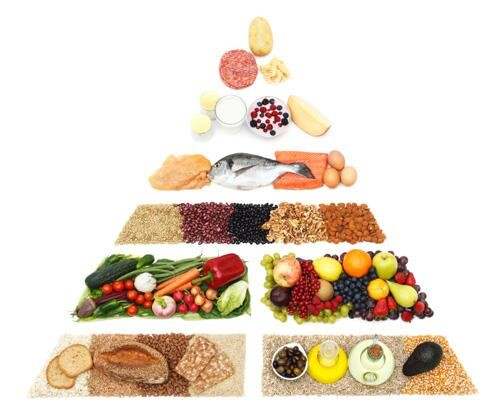
\includegraphics[width=0.6\textwidth]{img/mediterranean_diet_pyramid.jpg}
\end{center}


\textbf{Пирамида средиземноморской диеты.} Орехи – неотъемлемая часть средиземноморской диеты. Но поскольку они высококалорийные, желательно съедать в день не больше горсточки, которая помещается в одной ладони. Также средиземноморская диета содержит много бобовых. Постарайтесь постепенно вводить в свой рацион бобовые – фасоль, нут, горох, чечевицу. На их основе можно готовить супы и другие блюда.

Основной источник жиров в средиземноморской диете – это оливковое масло, которое содержит мононенасыщенные жиры. Если заменить насыщенные жиры (сливочное масло, мясо и т.п.) оливковым маслом, в организме снижается уровень «плохого» холестерина – липопротеидов низкой плотности. Лучше использовать оливковое масло, прошедшее наименьшую обработку, – «extra-virgin» и «virgin». Оно содержит максимум антиоксидантов.

Средиземноморскую диету невозможно представить без рыбы и морепродуктов. Жирная рыба (скумбрия, радужная форель, сардина, лосось, сельдь) богата на омега-3 жирные кислоты, полезные для здоровья кожи и сердечно-сосудистой системы. Средиземноморская диета предполагает умеренное употребление яиц и молочных продуктов – сыров и йогурта. Желательно выбирать продукты с низким содержанием жиров. Красное мясо появляется на столе всего лишь 1-2 раза в месяц. Это не повседневная еда, а, скорее, деликатес, которым можно себя изредка побаловать.


Некоторые научные исследования указывают на то, что умеренное употребление вина снижает риск заболеваний сердца. Но при этом важно понимать, что такое «умеренное употребление». Для женщин – это 150 мл (1 бокал) вина, а для мужчин – 300 мл (2 бокала) в день. При этом дневные дозы нельзя «накапливать». Если вы не пили всю неделю, это не означает, что на выходных можно опустошить всю бутылку.

Попробуйте средиземноморскую диету. Она не предполагает резкого ограничения килокалорий и не вызывает чувство голода. Замените красное мясо рыбой и птицей, сливочное масло – оливковым маслом, сладости – фруктами и орехами. Это простой и безопасный путь к здоровью.

\textbf{Комментарий врача Универсальной клиники «Оберіг»:} Средиземноморская диета является универсальной для профилактики и лечения большинства возрастных болезней цивилизационного мира.

Кроме общеизвестной пользы Омега-3 жирных кислот, которые содержатся преимущественно в морской рыбе, один из важнейших принципов заключается в ежедневном употреблении полезных растительных жиров, которые содержатся в оливковом масле и расширение ежедневного рациона за счет овощей, салатов.

Скажете, что данные принципы можно соблюдать только в странах Средиземноморья и только в летний период? На самом деле, в украинских традициях тоже возможна вкусная и полезная модификация. Так, Омега-3-ненасыщенные жирные кислоты содержатся также в семенах тыквы, льна, грецких орехах и арахисе, бобовых, яйцах, шпинате, капусте и мяте. В зимнее время года полезным будет употребление украинских аналогов средиземноморской диеты – свекольно-морковных салатов, овощных супов, винегрета (исключая картофель), при этом оливковое масло первого отжима можно заменить на нерафинированное подсолнечное, льняное, рапсовое, горчичное или соевое.


Соблюдение данных принципов способствует регулярной эвакуации желчи, нормализует работу желудочно-кишечного тракта, налаживает метаболизм, уменьшает уровень холестерина и риски сердечно-сосудистых осложнений.




\section{Курение вредит вашему здоровью}
Источник: \url{https://novo-sibirsk.ru/news/266296/}

Основным веществом для табачных изделий является никотин. В равных количествах он более ядовит, чем стрихнин, и обладает в 3 раза большей токсичностью, чем мышьяк. Табачный дым в 4,5 раза токсичнее автомобильных выхлопов и в 248 раз - дыма газовой горелки.

К настоящему времени в табачных изделиях обнаружено около 4000 химических соединений, а в табачном дыме около 5000, из них около 60 веществ являются известными или предполагаемыми канцерогенами.

Смертельная доза для взрослого человека 60 мг никотина, а для детей еще меньше.

В невыкуренной сигарете содержится порядка 10 мг никотина, но через дым курильщик получает от одной сигареты порядка 3 мг никотина.

Главная опасность никотина заключается в том, что никотиновая зависимость поддерживает потребление табака. Никотиновая зависимость формируется очень быстро. Как правило, многие молодые курильщики недооценивают риск развития зависимости. Однако 98\% регулярных курильщиков, пробующих отказаться от курения, терпят неудачу сразу или начинают курить снова в течение года.

Температура табачного дыма, поступающего в рот при курении, на 35-40 градусов выше температуры воздуха и вызывает во рту довольно резкий перепад температур. Во время курения одной сигареты происходит 15-20 таких перепадов, что плохо отражается на состоянии зубной эмали: она трескается. Вот почему зубы курильщика разрушаются раньше, чем зубы некурящих.

При выкуривании 1 пачки сигарет курильщик производит около 1 грамма жидкого дегтя, который оседает на пальцах, в бронхах, легких, попадает в желудок.

Курение приводит к развитию трех основных заболеваний с летальным исходом: рак легкого; хронический бронхит и эмфизема; коронарная болезнь. 90\% онкологических заболеваний вызвано курением табака. Подсчитано, что у людей, начавших курить с 15-летнего возраста, он возникает в 5 раз чаще, чем у тех, кто закурил позже 25 лет. Продолжительность жизни курящего человека сокращается на 20-25 лет.

При выкуривании 20 сигарет в день за год курильщик получает дозу облучения, соответствующую дозе от 200 рентгеновских снимков.

У молодых курящих женщин поражаются вены нижних конечностей с последующим развитием у них эктазий, варикоза, тромбозов. Наблюдается повышенный риск возникновения ишeмической болезни сердца, инфаркта миокарда, мозгового инсульта, частота развития которого в 20 раз выше, чем у некурящих.


\section{Вред алкоголя, его влияние на организм человека }

Источник: \url{http://pol1.tomsk.ru/novosti/281-21-09-2018}

Алкоголь – штука коварная: с одной стороны, бокал пива – просто незаменимое лекарство от перенапряжения после тяжелой рабочей недели. Но с другой – это невидимый, но достаточно ощутимый удар по здоровью, бьющий в самые уязвимые места нашего организма.

О семи причинах, почему стоит отказаться от алкогольных напитков и о том, как они способны навредить твоей жизни – далее в нашей статье.

1. Удар по сердечно-сосудистой системе. Как только алкоголь попадает в организм, сердце начинает увеличиваться в размере (особую коварность таит в себе пиво). На тканях сердца появляются многочисленные рубцы, которые являются виновниками инфаркта и способны привести к смерти.

2. Затуманенный рассудок. Алкоголь не зря считается разновидностью наркотических веществ: спиртные напитки оказывают на психику эйфорическое воздействие, продолжительность которого составляет от часа до полутора. Вскоре после этого человек впадает в депрессивное состояние, сопровождающееся агрессией и приступами панического страха. Реакции снижаются, о ясном мышлении в такой ситуации не может быть и речи. Именно по этой причине, как известно, водителям нельзя пить: вождение в нетрезвом виде может закончиться самым плачевным исходом.

3. Уничтожение клеток мозга. Даже небольшое количество алкоголя (да, полбокала вина также сюда относится) уничтожает несколько тысяч нейронов без возможности восстановления. Спирт, содержащийся в алкогольных напитках, провоцирует склеивание эритроцитов – красных кровяных телец: последние закупоривают микрокапилляры, приводя к смерти нейронов от кислородного голодания. Клетки, павшие в неравном бою с алкоголем, выводятся из организма с мочой.

4. Развитие хронических болезней. Медики приравнивают действие алкоголя к медленному яду: продукты распада спирта разрушают организм в прямом смысле слова. Человек, регулярно употребляющий спиртное, со временем все чаще начинает ощущать недомогание, его умственная и физическая активность заметно снижаются, на смену им приходит апатия. Длительная алкогольная зависимость – залог развития таких опасных хронических болезней, как панкреатит, рак поджелудочной железы, цирроз, инфаркт и масса других коварных заболеваний. Не самая обнадеживающая перспектива, не так ли?

5. Плохая наследственность. Алкоголь вносит изменения в структуру генетического кода ДНК – именно она содержит в себе информацию о человеке и его потомках. Ученые давно пришли к выводу, что 90\% детей с отклонениями в умственном развитии и врожденных инвалидов рождаются у людей, злоупотребляющих спиртными напитками.

6. Непристойное поведение. Уверены, тебе не раз приходилось наблюдать, что из себя представляет пьяный человек: алкоголь оказывает влияние на нравственные центры головного мозга, в связи с чем его дальнейшее поведение становится абсолютно непредсказуемым. В лучшем случае, все заканчивается мирным посапыванием в укромном уголке. В худшем – неконтролируемой агрессией, вспышками гнева и другими малоприятными вещами, которые в трезвом виде человек ни за что бы себе не позволил.

7. Дыра в бюджете. Цены на алкоголь (особенно хороший) немалые, и регулярное распитие любимых спиртных напитков зачастую влетает в немалую копеечку. К тому же, люди, которые начали испытывать зависимость от алкоголя, на одной бутылке не останавливаются: чем сильнее “захмелевает” голова, тем больше напитка будет куплено. Даже банальный просмотр футбольного матча практически никогда не обходится без нескольких банок пива – что уж говорить о пикнике с компанией, рыбалке или дне рождения. Если подсчитать, в какую сумму обходится такой досуг, действительно возникнет желание отложить эти деньги для более разумных целей (вложить в путешествие или же, к примеру, порадовать себя новым гаджетом).

Как видишь, существует масса причин как можно реже притрагиваться к спиртному, а то и вовсе от него отказаться. Да, алкоголь создает эффект расслабления. Да, он раскрепощает и снимает внутренние зажимы. Но тот вред, который организм получает параллельно, сводит “на нет” и без того небольшие преимущества. К тому же, расслабиться можно и другими способами – йога, плавание, горячая ванна, сауна, массаж или же неспешная прогулка в спокойном зеленом парке являются лучшими помощниками в этом деле. Позаботься о собственном здоровье сейчас, и в будущем у тебя будет в разы больше шансов избежать больничной койки и массы других малоприятных “бонусов”, нажитых за годы употребления алкоголя.

\section{Восемь советов как избежать стресса}
Источник: \url{https://primamedia.ru/cards/health04/}

Суетливая повседневность, напряженность, проблемы, которые ежедневно нас беспокоят, нарушают наше психическое равновесие и спокойствие. Эксперты убеждены, что для эффективного управления стрессом мы должны быть достаточно мотивированы и сами выстраивать стратегию, которая поможет нам в трудные времена.

Эти советы могут быть полезны при нашем повседневном стрессе - они усилят энергию и поддержат жизненный тонус.

\textbf{1. Лестница вместо лифта.}
Когда мы пребываем в унынии, то частенько «успокаиваем» себя конфетами, сигаретой или чашечкой кофе. Гораздо лучшим вариантом является физическая активность.

В состоянии стресса или гнева попробуйте больше двигаться. Можно подняться по лестнице или совершить быструю прогулку. Даже 10 минут упражнений улучшат настроение и повысят энергетику.

\textbf{2. Еда снижает стресс. Миф! Насытьте себя «воздушной смесью».}
Вы пытаетесь снять стресс пищей? Многие считают, что это приносит комфорт, по крайней мере, в краткосрочной перспективе. Самообман.

В напряженные моменты ешьте фрукты или овощи. Это хоть предотвратит накопление лишних килограммов.

Попробуйте вместо еды, в стрессовой ситуации, сделать несколько глубоких вдохов.

\textbf{3. Полноценный сон делает нас более гармоничными.}
Качество сна – это способ борьбы с нервными состояниями. Нужно 7-9 часов сна, чтобы уменьшить стресс и подзарядиться для следующего дня.

Если у вас проблемы с засыпанием, ограничьте потребление кофеина. Избегайте тренировки за два часа до сна. Удалите из своей спальни телевизор, домашних животных, компьютер и другие «отвлекашки».

\textbf{4. Выбирайтесь из рутины.}
Даже небольшие изменения в повседневной жизни помогут улучшить настроение.

Найдите другие маршруты для похода на работу или прогулки с собакой. Измените меню завтрака или ужина.

Сосредоточьтесь на легко достижимых изменениях, чтобы добиться гарантированного успеха.

\textbf{5. Прогулка по окрестностям.}
Вам не нужно часами пыхтеть в тренажерном зале. Даже небольшие телодвижения могут быть полезны для восстановления вашей энергетики.

Простая прогулка по ближайшему скверику поможет освежить ум. Упражнения на свежем воздухе, включающие медитацию, йогу или ци-гун, помогают зарядить не только ум, но и тело.

\textbf{6. Больше волокнистой пищи!}
Получение достаточного количества клетчатки полезно для улучшения пищеварения и поддержания здоровья сердца.

Много волокон находится в овсяной муке, цельнозерновом хлебе и крупах, овощах и фруктах (в яблоках, клубнике, цитрусовых).

\textbf{7. Сосредоточьтесь на сегодняшнем дне.}  Оставьте свои мысли о прошлом или будущем, сосредоточьтесь на текущем моменте. Важно знать, где вы находитесь именно сейчас! Направьте свою энергию на то, что вы делаете в данный момент! Насладитесь тем, что с вами происходит!

\textbf{8. Не пренебрегайте здоровьем.} Мы стараемся игнорировать головную боль, «раздражающий» кашель, усталость или другие лёгкие недомогания. Но это всё влияет на наше психическое состояние, включая нашу жизнеспособность. Поэтому в случае симптомов и подозрений по поводу здоровья, рекомендуется своевременно обратиться к врачу.

Полезно внимательно слушать и уважать себя и свой организм!


\section{Диабет}
Источник: \url{https://www.who.int/ru/news-room/fact-sheets/detail/diabetes}

\textbf{Основные факты.}
\begin{enumerate}
    \item За период с 1980 по 2014 г. количество людей, страдающих диабетом, выросло со 108 миллионов до 422 миллионов. В странах с низким и средним уровнем дохода распространенность диабета растет быстрее, чем в странах с высоким уровнем дохода.
    \item Диабет является одной из ведущих причин слепоты, почечной недостаточности, сердечных приступов, инсульта и ампутации нижних конечностей.
    \item С 2000 по 2016 г. преждевременная смертность от диабета увеличилась на 5\%.
    \item В 2019 г. диабет стал девятой ведущей причиной смерти в мире и, согласно оценкам, непосредственной причиной 1,5 миллиона случаев смерти.
    \item Здоровое питание, регулярная физическая активность, поддержание здоровой массы тела и воздержание от употребления табака могут предупредить или отсрочить возникновение диабета 2-го типа.
    \item Диабет поддается лечению, а диета, физическая активность, медикаментозное лечение и регулярный контроль и лечение осложнений помогают предупредить или задержать наступление его последствий.
\end{enumerate}

Диабет — хроническая болезнь, развивающаяся в тех случаях, когда поджелудочная железа не вырабатывает достаточно инсулина или когда организм не может эффективно использовать вырабатываемый им инсулин. Инсулин — это гормон, регулирующий уровень содержания сахара в крови. Распространенным следствием неконтролируемого диабета является гипергликемия, или повышенный уровень содержания сахара в крови, со временем приводящая к серьезному повреждению многих систем организма, особенно нервов и кровеносных сосудов.

В 2014 г. заболеваемость диабетом среди взрослого населения в возрасте 18 лет и старше составляла 8,5\%. В 2019 г. диабет стал непосредственной причиной 1,5 миллиона случаев смерти, и 48\% всех связанных с диабетом случаев смерти произошли в возрасте до 70 лет.

С 2000 по 2016 г. преждевременная (т. е. в возрасте до 70 лет) смертность от диабета увеличилась на 5\%. В странах с высоким уровнем дохода показатель преждевременной смертности от диабета снижался с 2000 по 2010 г., но затем вновь увеличился в 2010–2016 гг. В странах с уровнем дохода ниже среднего прирост преждевременной смертности от диабета имел место в оба этих периода.

По сравнению с этим, за период с 2000 по 2016 г. вероятность наступления смерти в возрасте от 30 до 70 лет по причине неинфекционных заболеваний, принадлежащих к одной из четырех основных групп (сердечно‑сосудистые, онкологические, хронические заболевания органов дыхания или диабет), снизилась во всем мире на 18\%.

\textbf{Диабет 2‑го типа.} Диабет 2‑го типа (ранее — инсулиннезависимый или диабет взрослых) развивается в результате неэффективного использования инсулина организмом. Диабетом 2‑го типа страдает более 95\% диабетиков. Данный тип диабета возникает, главным образом, на фоне избыточной массы тела и недостаточной физической активности.

Его симптомы могут быть сходными с симптомами диабета 1‑го типа, но часто менее выражены. В результате болезнь нередко диагностируется по прошествии нескольких лет после ее возникновения, уже после появления осложнений.

До недавнего времени диабет этого типа наблюдался лишь среди взрослых, однако в настоящее время он все чаще поражает и детей.

\textbf{Диабет 1‑го типа.} При диабете 1‑го типа (ранее – инсулинозависимый, юношеский или детский), для которого характерна недостаточная выработка инсулина, пациенту требуется ежедневное введение инсулина. В 2017 г. в мире было зарегистрировано 9 миллионов больных диабетом 1‑го типа, причем большинство из них проживали в странах с высоким уровнем дохода. В настоящее время причина этого типа диабета неизвестна, а меры профилактики не разработаны.

Симптомы включают чрезмерное мочеотделение (полиурия), жажду (полидипсия), постоянное чувство голода, потерю веса, нарушения зрения и усталость. Эти симптомы могут появиться внезапно.

\textbf{Гестационный диабет.} Гестационный диабет проявляется гипергликемией с показателями глюкозы крови, которые превышают нормальные, однако не достигают диагностически значимых для постановки диагноза диабета. Гестационный диабет имеет место во время беременности.

Женщинам с такой формой диабета угрожает повышенный риск осложнений во время беременности и родов. Они и, возможно, их дети подвергаются повышенному риску дальнейшего развития диабета 2‑го типа.

Чаще всего гестационный диабет диагностируется не по жалобам пациентки, а при проведении пренатального скрининга.
Снижение толерантности к глюкозе и нарушение гликемии натощак

Пониженная толерантность к глюкозе (ПТГ) и нарушение гликемии натощак (НГН) являются промежуточными состояниями между нормой и диабетом. Люди с ПТГ и НГН подвергаются высокому риску развития диабета 2‑го типа, однако этого может и не произойти.


\textbf{Последствия диабета для здоровья.}
Со временем диабет может приводить к поражению сердца, кровеносных сосудов, глаз, почек и нервов.

У взрослых людей с диабетом в 2–3 раза выше риск развития инфаркта и инсульта (1).

В сочетании со снижением кровотока невропатия (повреждение нервов) нижних конечностей повышает вероятность появления на стопах язв, инфицирования и, в конечном счете, необходимости ампутации.

Диабетическая ретинопатия, являющаяся одной из важных причин слепоты, развивается в результате долговременного накопления повреждений мелких кровеносных сосудов сетчатки. С диабетом связан почти один миллион случаев слепоты во всем мире (2).

Диабет относится к числу основных причин почечной недостаточности (3).

\textbf{Профилактика.} Известно, что простые меры по поддержанию здорового образа жизни способствуют профилактике диабета 2‑го типа либо позволяют отсрочить его возникновение. Для повышения шансов на предупреждение диабета 2‑го типа и связанных с ним осложнений, необходимо:

добиться здоровой массы тела и поддерживать ее; поддерживать физическую активность — по меньшей мере 30 минут регулярной активности умеренной интенсивности в течение большинства дней; для контроля веса необходима дополнительная активность; придерживаться здорового питания и уменьшать потребление сахара и насыщенных жиров; и не употреблять табак — курение повышает риск развития сердечно-сосудистых заболеваний.


\section{Пять причин делать утреннюю зарядку}
Источник: \url{https://med-atlant.ru/news/5-prichin-delat-utrennyuyu-zaryadku/}

Утреннее пробуждение всегда сопряжено с сонливостью и даже некоторой ленью. Чтобы взбодриться, некоторые люди тут же заваривают себе ароматный кофе, другие начинают день с принятия душа. И только немногие пробуждаются при помощи утренней зарядки. Как показывает практика, именно те, кто взбадривает организм физкультурой, быстрее переходят в активный режим. Итак, в чем же польза зарядки? Для чего она нужна? И какие упражнения лучше делать по утрам?

Приходилось ли вам замечать, как много людей утром в плохом настроении? Врачи считают, что одна из причин такого состояния заключена в гипокинезии. Иными словами, в отсутствии физической активности. Ничего удивительного. Проработанные мышцы посылают в головной мозг достаточное количество импульсов, благодаря которым он активно настраивается на рабочий лад.

Люди, которые отказываются от утренней зарядки, часто страдают от нервной возбудимости, испытывают хроническую усталость. Они жалуются на отсутствие энергичности и бодрости утром. И только к полудню такие люди отмечают повышение активности.

\textbf{Зачем нужна зарядка.}
Организм человека не способен полностью пробудиться по звонку будильника. И даже в тот момент, когда вы уже поднялись с кровати, все внутренние органы и системы еще продолжают «отдыхать».

Во время сна замедляется циркуляция крови, затормаживается метаболизм, снижается умственная деятельность. Именно поэтому во время пробуждения человек ощущает легкую заторможенность. У него отмечается сниженная работоспособность, как физическая, так и умственная. Утром значительно ухудшена скорость реакций.

Такое состояние может длиться (в зависимости от индивидуальных особенностей) от 1 до 3 часов. Чтобы полностью проснуться и стряхнуть подобную «заторможенность», необходимо разработать суставы и мышцы. Другими словами, нужно просто сделать зарядку.

\textbf{Какая польза от зарядки?}
С самого детства родители твердили нам о необходимости делать зарядку. Лишь немногие безропотно прислушались к таким рекомендациям. А большая часть людей, прежде чем начать делать утреннюю зарядку, стремится понять, что же такого ценного она приносит.

Физическая активность в утреннее время обеспечивает следующее.

\textbf{Придает бодрость.} Организм человека просыпается значительно быстрее и активнее, если была совершена даже небольшая зарядка. После физкультуры активизируется кровообращение. Все органы и ткани начинают активно насыщаться кислородом. Ощущается прилив энергии, улучшается самочувствие. Мозг, получивший свою порцию кислорода, активно включается в рабочий процесс.


\textbf{Улучшает физическую форму.} Регулярные занятия приводят к укреплению мышечных тканей. Физкультура положительно влияет на состояние позвоночника и суставов. Даже простая и недлительная гимнастика служит отличной профилактикой развития многих болезней опорно-двигательного аппарата.

Утренняя зарядка стимулирует метаболизм. Благодаря этому человек постепенно обретает красивые формы. Некоторые мышцы подкачиваются, появляется стройность, подтягивается живот.

\textbf{Повышает настроение.} Зачем делать зарядку, если можно взбодриться от чашки кофе? Увы. Это не так. Ароматный напиток не обеспечит той энергичности и позитива, которые подарит утренняя гимнастика.

Зарядка подразумевает набор простых упражнений, которые направлены на разогрев мышц и проработку суставов. Никаких чрезмерных нагрузок утренняя физкультура не содержит. А поэтому она не вызывает ощущения усталости или боли.

\textbf{Укрепляет силу воли.}   Приняв решение делать зарядку, вам необходимо заставить себя подниматься на 10-15 минут раньше. На первых порах при правильном настрое и соответствующей мотивации вы с легкостью преодолеете этот барьер.

Но со временем, приблизительно к 20-21 дню, могут начаться серьезные трудности. Положительные результаты к этому времени еще мало заметны. Поэтому начинают появляться навязчивые мысли: «Зачем мне нужна эта зарядка, она все равно ничего не дает. Лучше поспать лишние 10-15 минут». Вот именно в этот момент важно не поддаться таким мыслям и преодолеть себя. Такое «упражнение» здорово прокачает вашу силу воли.

\textbf{Укрепляет здоровье.}
Утренняя зарядка оказывает комплексное воздействие на организм. Она активизирует кровообращение, ускоряет обмен веществ. Благодаря улучшенному кровотоку все внутренние органы получают достаточное питание и начинают значительно активнее функционировать.

Польза утренней зарядки заключена в следующих воздействиях:

\begin{itemize}
    \item укрепление сердечной мышцы;
    \item улучшение работы дыхательной системы;
    \item повышение упругости мышц;
    \item нормализация состояния сосудов, повышение их проходимости;
    \item выравнивание осанки;
    \item усиление концентрации внимания;
    \item повышение подвижности суставов;
    \item стимуляция работы мозга;
    \item повышение выносливости;
    \item нормализация работы вестибулярного аппарата.
\end{itemize}

\textbf{Утренняя зарядка: основные правила и рекомендуемые упражнения.} Существует еще одно распространенное заблуждение. Некоторые люди уверенны, что не обязательно делать зарядку утром. Можно практиковать физическую активность после обеда и даже вечером. Если речь идет об утренней зарядке, то все специалисты сходятся в одном: она должна быть утром, после пробуждения. Ведь основная цель такой гимнастики – зарядить человека бодростью и энергией на весь день.

\section{Пять важных рекомендаций}
Источник: \url{https://med-atlant.ru/news/5-prichin-delat-utrennyuyu-zaryadku/}

Чтобы польза зарядки, выполняемой  по утрам, была максимальной, необходимо соблюдать следующие правила.

\textbf{Продолжительность гимнастикию.} Тем, кто только начинает вводить в свою жизнь утреннюю зарядку, рекомендуется планировать 10-минутную физкультуру. Со временем можно увеличить время до 15 минут. Когда организм полностью адаптируется к нагрузкам (приблизительно через 3-6 месяцев) начинайте увеличивать время зарядки до получаса.

\textbf{Подготовка к зарядке.} Не стоит приступать к гимнастике сразу после подъема с кровати. Организм еще продолжает спать. Такие нагрузки вызовут дискомфорт. Изначально нужно немного взбодриться. Для этого рекомендуется умыться, почистить зубы.

Обязательно выпейте стакан воды. Жидкость, поступившая в организм, обеспечит разжижение крови. Благодаря этому удастся нормализовать нагрузку на сердце и сосуды. А вот перекусывать перед зарядкой не стоит. Все упражнения выполняйте натощак.

\textbf{Добавьте эмоции.} Зарядка должна не только взбадривать, но и повышать настроение. Поэтому включайте любимую музыку, насыщайте воздух ароматными маслами (только не переусердствуйте) и занимайтесь гимнастикой. После физкультуры обязательно хвалите себя, отмечайте все достижения и не забывайте о поощрении.

Чтобы зарядка принесла значительную пользу для организма, предварительно проветрите помещение. Это можно сделать в то время, пока вы умываетесь. Приток свежего воздуха позволит насытить организм большим количеством кислорода.

\textbf{Регулярность занятий.} Если вы делаете зарядку от случая к случаю, то надеяться на положительные результаты не стоит. Пользу принесут только ежедневные занятия. Причем первые результаты станут заметны через 5-6 недель регулярных тренировок.

В это время люди обычно отмечают снижение уровня стресса, позитивный настрой, уменьшение возбудимости и раздражительности. Практикующие утреннюю зарядку утверждают, что к 5-6-й неделе усиливается работоспособность, повышается дисциплинированность и упорство. Люди становятся крепче и практически не подхватывают простуды.

\textbf{Правильный комплекс.} Еще один важный момент, который не следует упускать из виду, – это правильный комплекс упражнений. Гимнастика должна «запустить» все органы и ткани. Именно поэтому комплекс составляйте из упражнений, прорабатывающих все мышцы и суставы.



Утренняя зарядка должна включать в себя три этапа:
\begin{enumerate}
    \item Разминку. Ее можно делать лежа в постели. Она включает потягивание, дыхательные упражнения. В этот комплекс могут входить легкие вращательные движения кистями, стопами, конечностями.
    \item Основной комплекс. Он состоит из упражнений, прорабатывающих все мышцы и суставы. Начинают обычно с шеи, затем переходят на плечи, верхние конечности. Теперь очередь подходит к мышцам спины, живота. Заканчивают основной комплекс махами ногами.
    \item Завершение, или заминку. После основного комплекса рекомендована ходьба на месте и дыхательные упражнения.
\end{enumerate}



\section{Рекомендуемые упражнения}
Источник: \url{https://med-atlant.ru/news/5-prichin-delat-utrennyuyu-zaryadku/}

Особое внимание следует обратить на интенсивность нагрузок. Утренняя зарядка должна приносить пользу и заряжать энергией, а не истощать организм. Именно поэтому от тяжелых упражнений (с гантелями, штангой, на выносливость и т. д.) нужно отказаться. Интенсивные тренировки лучше всего проводить после обеда. А утром отдайте предпочтение легким, простым движениям.

Утренняя зарядка обычно включает следующие группы упражнений:
\begin{enumerate}
    \item \textit{Дыхательная гимнастика}. Она улучшает работу дыхательной системы и обеспечивает активный приток кислорода к внутренним органам.
    \item \textit{Ходьба}. Очень полезно ходить босыми ногами по полу. В этом случае массируются многие активные точки. Специалисты по нетрадиционной медицине утверждают, что именно на стопе их больше всего.
    \item \textit{Гимнастика для шеи}. Она включает повороты и наклоны головы. Такие упражнения должны выполняться очень осторожно, без надрывов. Полезны вращательные движения головой. Они не только укрепляют мышцы шеи, но и тренируют вестибулярный аппарат.
    \item \textit{Физкультура для верхних конечностей}. Обязательно выполняйте упражнения на поднятие рук вверх, разведение в стороны. Вращайте конечностями. Это способствует вытягиванию позвоночника и укреплению плечевого пояса.
    \item \textit{Упражнения для кистей и пальцев}. Такие занятия полезны тем людям, работа которых связана с руками (операторы ПК, музыканты, художники, ювелиры). Эта гимнастики активизирует кровообращение и укрепляет суставы.
    \item \textit{Физкультура для поясничного отдела}. В утреннюю зарядку нужно включать наклоны в разные стороны, вперед/назад. Если нет особых проблем с позвоночником, рекомендованы упражнения на скручивания. Полезны вращательные движения талией.
    \item \textit{Приседания}. Они повышают подвижность коленных и тазовых суставов. Кроме того, такие простые упражнения позволяют улучшить внешний вид икр и бедер.
    \item \textit{Упражнения на пресс}. Если вам совершенно не дает покоя животик или очень хочется сформировать рельефные кубики на животе, то включите в зарядку упражнения на пресс.
    \item \textit{Махи ногами и руками}. Такая гимнастика повышает тонус мышечных тканей и ускоряет кровообращение.
    \item \textit{Бег, прыжки}. Эти движения отлично прорабатывают все мышцы нижних конечностей. Кроме того, они значительно усиливают метаболизм.
\end{enumerate}
Если строгие комплексы навевают на вас тоску, то можете придумать свои собственные упражнения. Главное, чтобы они не истощали вас и прорабатывали все мышцы. Кстати, никто не запрещает вам просто танцевать под любимую музыку, периодически поднимая руки, совершая махи ногами и работая талией.


\section{Зачем нам нужны фрукты и овощи? Основы здорового питания!}
\textit{Автор: Юлия Баяндина.
    Источник: \url{https://www.shkolazhizni.ru/health/articles/63634/}}

С самого детства мы только и слышим — нужно есть свежие фрукты и овощи, в них много витаминов, они очень полезные. А почему? Этого никто не объясняет. Давайте разберемся, что нам это дает, и в чем состоит польза фруктов и овощей.

1. Поднимают настроение
Фрукты и овощи сродни шоколаду — содержат вещества (селен и фолиевую кислоту), которые способствуют выработке эндорфинов. Если что-нибудь не задалось — съешьте яблоко или банан, и настроение улучшится.

2. Дарят бодрость Фрукты и овощи содержат много воды — одновременно спасают и от голода, и от жажды, быстро усваиваются. Если нужен заряд бодрости — лучшего решения не найти. Поэтому утренний завтрак так полезно начинать с фруктов — и настроение поднимут, и энергией зарядят.

3. Добавляют витаминов Сколько фармацевты ни бьются над созданием супервитаминок, а идеального баланса найти не могут. Невозможно в одной таблетке уместить витамины так, чтобы все они полностью усваивались! С овощами и фруктами такой проблемы не возникает — все гармонично, все усваивается.

4. Помогают похудеть Овощи и фрукты содержат море клетчатки, которая почти не содержит калорий, но дает ощущение сытости. Поэтому их можно есть в любом количестве и не бояться лишнего веса — ему при таком рационе неоткуда будет взяться. Вдобавок клетчатка, словно липкая лента, собирает вредные химические вещества и канцерогены и выводит их из организма.

5. Спасают от холестерина Ничто так не страшно для сердечно-сосудистой системы, как избыток холестерина. Снизить его уровень в крови тоже помогут фрукты и овощи. Холестерин попадает в организм с животной пищей и вырабатывается печенью. В растительной пище холестерина нет, зато в ней есть пектин, который помогает выводить вредный холестерин из организма.

6. Продлевают молодость Помните молодильные яблочки из сказок? Так вот — они существуют. Сырые овощи и фрукты содержат антиоксиданты, которые помогают обновляться клеткам организма и предотвращают окисление органических соединений — попросту говоря, позволяют вам быть моложе и свежее.

7. Делают умнее Овощи и фрукты помогут сохранить ясность ума и отличную память: недавно опубликовали результаты исследования, в котором выяснили, что 6-8 фруктов и овощей в день помогают лучше запоминать и решать математические задачки. А еще фрукты и овощи спасают от заболеваний мозга: в знаменитой книге «Китайское исследование» пишут, что три порции фруктов и овощей каждый день помогут снизить риск инсульта. Одна порция -- это, к примеру, $\nicefrac{1}{2}$ чашки персиков, $\nicefrac{1}{4}$ чашки томатного соуса, $\nicefrac{1}{2}$ чашки брокколи или одна картофелина. Полчашки -- это немного.

8. Защищают от болезней Ученый Колин Кэмбелл 20 лет искал взаимосвязь между болезнями и питанием. Проверил рацион миллионов людей и доказал — фрукты и овощи лечат лучше любого доктора. Аргумент. И чем больше их в вашем рационе — тем ниже риск заболеть раком, диабетом и прочими страшными болезнями. Факт.

9. Экономят время Потому что их практически не надо готовить. Конечно, есть картофель сырым не стоит, но большинство фруктов перед едой достаточно просто вымыть. И в конце концов, фрукты и овощи — это просто очень вкусно!

% % Автор: Юлия Баяндина
% % Источник: https://www.shkolazhizni.ru/health/articles/63634/
% % © Shkolazhizni.ru


\section{Лекарство от всех болезней, кроме смерти}
\textit{Источник: \url{https://lenta.ru/articles/2022/09/24/tmin/}}

\textit{Что говорят врачи о пользе и вреде масла черного тмина}

Семена черного тмина использовали еще в Древнем Египте три тысячи лет назад. Во время раскопок одной из гробниц археологи обнаружили бутылочку с маслом, и последующая экспертиза установила, что его изготовили из тмина. Египтяне использовали масло как один из компонентов противоядия от укусов змей, как косметическое средство и глистогонный препарат, а также употребляли в пищу для улучшения пищеварения и работы почек и печени. Как используют черный тмин и масло из него в XXI веке, «Лента.ру» разбиралась с экспертами.

Масло черного тмина имело популярностью не только в Египте. О его свойствах писали в медицинских трактатах великие древние греки Диоскорид и Гиппократ.

В арабском мире популярности масла, помимо его целебных качеств, способствовали слова, приписываемые пророку Мухаммеду. В Коране упоминается, что он называл семена тмина «лекарством от всех болезней, кроме смерти».

\textbf{Как получают масло черного тмина}

Масло черного тмина добывают путем холодного отжима семян чернушки посевной. Это однолетнее травянистое растение семейства лютиковых имеет еще несколько названий: калинджи, сейдана (седана), черный тмин, римский кориандр.

Родиной черного тмина считаются Средиземноморье и Юго-Западная Азия, где, к слову, произрастает большинство самых популярных специй. Но сейчас калинджи растет и в Крыму, и в Средней Азии, и на Балканском полуострове, и в других местностях.

Трава эта неприхотлива: всходит в степи, лесу, в садах и посевах. Черный тмин считается сорной травой, но ради семян его культивируют.

\begin{center}
    \Large
    Масло черного тмина имеет светло-желтый или зеленовато-коричневый оттенок, обладает пряным запахом и вяжущим, терпким вкусом
\end{center}

Масло черного тмина насыщено витаминами и минералами. Богатый полезными микроэлементами состав сделал его востребованным в фармакологии, кулинарии и косметологии.


\textbf{Состав масла черного тмина}

Масло черного тмина состоит из жирных кислот: арахиновой, омега-9 и омега-6, миристиновой, пальмитолеиновой и других. Если регулярно принимать масло черного тмина, то организм пополнится следующими витаминами:


\begin{itemize}
    \item витамины группы В. Оказывают положительное действие на работу ЦНС, улучшают обмен веществ, снижают риск развития анемии;
    \item витамин А. Помогает сохранять зрение, повышает защитные функции организма, улучшает обмен веществ;
    \item витамин E. Важен для сохранения беременности;
    \item витамин D. Снижает риск возникновения сердечно-сосудистых заболеваний, рахита. Укрепляет кости;
    \item аскорбиновая кислота. Повышает иммунитет, снижает уровень «плохого» \item холестерина, повышает физическую выносливость.
\end{itemize}

«Также в составе тминного масла есть каротиноиды, биофлавоноиды, фосфатидил, фитостеролы, восемь незаменимых аминокислот и важный активный компонент — тимохинон, который является мощным антиоксидантом с противовоспалительным, иммуномодулирующим и тонизирующим действием», — пояснила «Ленте.ру» терапевт клиники превентивной и антиэйдж-медицины Verba Mayr Мария Веригина.

\begin{fancyquotes}
    {\Huge 896 ккал}\\

    содержится в 100 граммах масла черного тмина
\end{fancyquotes}


\textbf{Польза масла черного тмина}

«Масло черного тмина помогает при язвенной болезни желудка, гастрите, энтерите, заболеваниях желчного пузыря и желчевыводящих путей, регулирует кислотность в желудке, — рассказала «Ленте.ру» диетолог Кристина Плотникова. — Но не стоит забывать, что это не лекарство, а сопутствующая вспомогательная терапия, и все заболевания должен лечить врач».

Масло черного тмина содержит вещества, которые могут снизить отечность, смягчить аллергические реакции, усилить иммунитет и даже отчасти помочь организму в борьбе с раковыми клетками.

Масло черного тмина имеет следующие свойства:

\begin{itemize}
    \item обезболивающее;
    \item противовоспалительное;
    \item антисептическое;
    \item бактерицидное;
    \item антивирусное;
    \item противопаразитарное;
    \item ранозаживляющее;
    \item антигрибковое;
    \item иммуностимулирующее.
\end{itemize}

\textbf{Воздействие масла черного тмина на организм}

Существует ряд исследований, доказывающих пользу масла черного тмина при лечении ряда недугов. Но стоит помнить, что его эффект пока не до конца изучен, а любая пищевая добавка не может заменить полноценного лечения под руководством опытного врача. Медики напоминают: не существует волшебной таблетки, и, если не вести здоровый образ жизни, любое средство, каким бы полезным оно ни было, не поможет справиться с последствиями вредных привычек.

\textbf{Помогает бороться с раком}

Исследования на животных показали, что семена черного тмина могут остановить рост опухолевых клеток и снизить частоту возникновения опухолей. Однако влияние на человека до конца не изучено.

\textbf{Снижает воспаление и боль при артрите}

Ученые опытным путем доказали, что микроэлементы, которые входят в состав масла черного тмина, способны улучшать состояние пациентов с ревматоидным артритом. Во время исследования части группы из 43 женщин с этим диагнозом давали масло, а остальным — плацебо. Через месяц у пациентов, принимавших масло черного тмина, зафиксировали снижение уровня маркеров воспаления крови, а также снижение интенсивности боли и уровня отека суставов.

\textbf{Защищает сердце и сосуды}

Масло черного тмина оказывает благотворное воздействие на сердце и сосуды. Оно является хорошим средством профилактики гипертонии, варикоза, тромбоза, ишемической болезни, атеросклероза.

\textbf{Помогает при аллергии}

Во время исследований в США установили, что масло черного тмина уменьшает отек в носу, заложенность носа, соответственно, помогает справиться с насморком. Правда, по данным исследования, чтобы добиться явного эффекта, масло нужно принимать две недели.

Масло черного тмина благодаря противовоспалительным и антигистаминным свойствам также способно снизить проявление аллергии и помочь быстрее избавиться от аллергического ринита.

\textbf{Избавляет от папиллом}

Бородавки и папилломы появляются на теле из-за попадания в организм вирусов. Масло черного тмина может избавить от новообразований.

Для этого нужно ватный или марлевый тампон смочить в подогретом тминном масле. Затем тампон разместить на пораженном участке кожи. Оставить его нужно на 5-6 часов, поэтому тампон следует закрепить пластырем или бинтом. Для полного избавления от бородавок и папиллом процедуру надо повторять каждый день в течение месяца.

Однако стоит помнить, что масло избавляет лишь от внешних проявлений болезни. Использовать его следует одновременно с медицинскими препаратами, назначенными врачом.

\textbf{Помогает бороться с диабетом}

Черный тмин помогает снизить уровень сахара и холестерина в крови. Люди, принимавшие добавки черного тмина, имели более низкий риск осложнений при сахарном диабете II типа. Однако это воздействие растения на организм человека предстоит изучить дополнительно.

\textbf{Поддерживает здоровье ЖКТ}

Ученые пришли к выводу, что тминное масло способно наладить процесс пищеварения и работу органов желудочно-кишечного тракта. Употребление масла помогает не только устранить причину развития заболеваний, но и убрать симптомы: приступы тошноты и рвоты, изжогу и колики.

К тому же масло тмина способствует заживлению повреждений слизистой оболочки желудка и ускорению процесса выздоровления.

\begin{fancyquotes}
    {\Huge 3-6 недель}\\

    нужно использовать тминное масло для появления ожидаемого эффекта
\end{fancyquotes}

\textbf{Помогает справиться с панкреатитом}

Принимать тминное масло можно только после наступления ремиссии заболевания и после консультации с врачом. В период обострения панкреатита масло может навредить.

После введения масла черного тмина в рацион снижается интенсивность проявления таких неприятных симптомов, как дискомфорт после приема пищи, отсутствие аппетита, метеоризм. К тому же масло останавливает размножение патогенных микроорганизмов и грибков.

\textbf{Предотвращает развитие рака простаты}

Ученые выяснили, что антиоксидант тимохинон способен подавлять рост раковых клеток в предстательной железе. Онкологи сходятся в мнении, что альтернативная медицина становится важной в качестве дополнительной терапии для больных раком, как для смягчения побочных эффектов химиотерапии, так и для усиления их противоопухолевых эффектов.

\textbf{Помогает бороться с простудой}

При простуде можно использовать масло черного тмина несколькими способами.

\begin{enumerate}
    \item Прием внутрь. Облегчить течение простуды поможет чай с тминным маслом. Но этот напиток является лишь дополнением к назначенной врачом терапии.
    \item Растирание. Грудную клетку можно растирать смесью из масла черного тмина и любого другого масла в пропорции 1:5 соответственно. Растирание поможет ослабить интенсивность кашля.
    \item Распаривание ног. Масло тмина обладает согревающим эффектом. Его добавляют в емкость с горячей водой, затем греют в ней ноги. Для большей эффективности в воду можно добавить порошок горчицы.
\end{enumerate}

\textbf{Избавляет от запора}

Тминное масло — отличное средство лечения и профилактики запоров. Оно улучшает перистальтику кишечника, размягчает каловые массы, выводит их без применения лекарственных препаратов. Особенно полезно масло как средство от запоров при беременности, во время грудного вскармливания, при нормализации стула у детей — в случаях, когда нежелательно пить лекарства.

Избежать запоров поможет масло черного тмина с чаем. Для этого нужно половину чайной ложки масла добавить в стакан чая и пить этот напиток дважды в день.

\textbf{Помогает людям с ожирением}

Масло черного тмина может помочь женщинам, страдающим ожирением. Во время исследований часть участниц научного эксперимента принимала плацебо, другая — масло. В конце исследования у участниц, принимавших масло, снизился вес, уменьшился обхват талии и уровень триглицеридов.

Исследователи также обнаружили, что сочетание диеты с приемом масла черного тмина и физическими упражнениями приводит к потере веса и снижению уровня холестерина.

Комментируя этот факт, эндокринолог клиники «РЖД-Медицина» в Твери Анна Куликова пояснила, что, согласно принципам рационального питания, следует ограничить прием всех растительных масел до столовой ложки в сутки (17 граммов). «Растительное масло, в том числе и масло черного тмина, — это на 99 процентов жир. Поэтому не стоит забывать о калорийности, ведь 100 граммов тминного масла — это почти 900 килокалорий!» — предупредила она.


\begin{fancyquotes}
    Масло черного тмина может оказывать положительное действие на организм. Входящие в его состав полезные вещества могут косвенным образом оказывать помощь в похудении. Но волшебной таблетки для избавления от лишнего веса не существует. 95-99 процентов случаев избытка массы тела связаны с перееданием и малой физической активностью.\\

    \begin{flushright}
        Анна Куликова, эндокринолог
    \end{flushright}
\end{fancyquotes}

\textbf{Облегчает состояние при астме}

Множество исследований черного тмина показали, что он облегчает состояние пациентов с бронхиальной астмой. Он оказал бронхолитическое, антигистаминное, противовоспалительное, антилейкотриеновое и иммуномодулирующее действие. Кроме того, клинические исследования установили, что при употреблении черного тмина улучшились лабораторные показатели анализов пациентов и работа легких.

\textbf{Спасает от паразитов}
Тминное масло стимулирует выработку лизоцима, способного остановить размножение глистов и других паразитов. Содержащиеся в масле элементы оказывают губительное воздействие не только на взрослых паразитов, но и их личинки.

Масло черного тмина действует следующим образом.

\begin{itemize}
    \item Убивает гельминтов, глистов, других паразитов, а также их яйца и личинки.
    \item Выводит паразитов из организма человека.
    \item Выводит из организма человека продукты жизнедеятельности паразитов — токсины.
    \item Восстанавливает пораженные паразитами ткани.
\end{itemize}

\textbf{Избавляет от геморроя}

Тминное масло входит в состав мазей и ванночек для лечения геморроя. Оно помогает снять или уменьшить болевой синдром, остановить кровотечение, упростить процесс дефекации, снять воспаление, повысить эластичность кожи и защитить ее от микротрещин.

Для избавления от геморроя нужно выпивать 2,5 миллилитра (чайная ложка) масла черного тмина утром и вечером. Но перед этим стоит проконсультироваться с врачом.

Также масло можно нанести на пораженный участок с помощью ватного тампона. Семена тмина можно добавлять в еду, смешивать с водой и медом.

[...]
